% "{'classe':('PSI'),'chapitre':'dyn_cin','type':('colle'),'titre':'Disque déséquilibré', 'source':'Équipe PT - La Martinière Monplaisir','comp':('C1-05','C2-09'),'corrige':False}"
%\setchapterimage{bandeau}
\chapter*{Colle \arabic{cptColle} \\ 
Disque déséquilibré -- \ifprof Corrigé \else Sujet \fi}
\addcontentsline{toc}{section}{Colle \arabic{cptColle} : Disque déséquilibré -- \ifprof Corrigé \else Sujet \fi}

\iflivret \stepcounter{cptColle} \else
\ifprof  \stepcounter{cptColle} \else \fi
\fi

\setcounter{question}{0}
\marginnote{Équipe PT -- PT$\star$ La Martinière Monplaisir.}
\marginnote{
\UPSTIcompetence[2]{C1-05}
\UPSTIcompetence[2]{C2-09}
}
%\begin{marginfigure}[4cm]
%\centering
%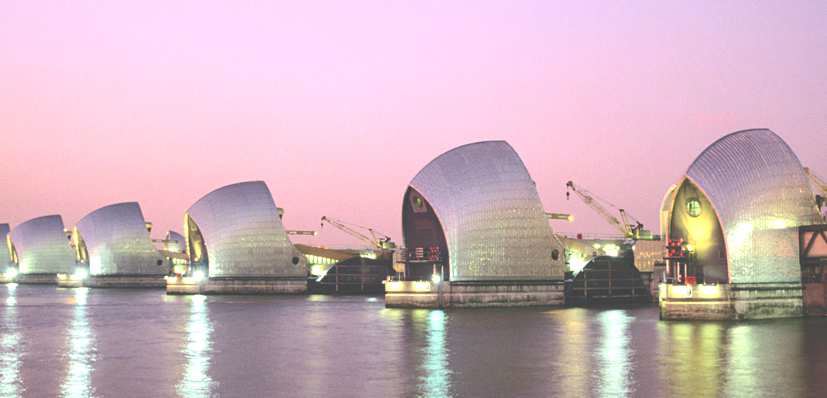
\includegraphics[width=.7\linewidth]{fig_00}
%\end{marginfigure}



Soit le rotor \textbf{(1)} défini ci-contre. Il est constitué d'un arbre de masse négligeable en liaison pivot par rapport à un bâti \textbf{(0)}. Sur cet arbre est monté, en liaison complète, un disque de masse $M$, de rayon $R$ et d'épaisseur $H$. 
Le repère $\mathcal{R}'_1=\repere{G}{x_1'}{y_1'}{z_1'}$ est attaché à ce solide.

La base $\mathcal{B}'_1=\base{x_1'}{y_1'}{z_1'}$ se déduit de $\mathcal{B}_1=\base{x_1}{y_1}{z_1}$  par une rotation d'angle $\alpha$ autour de $\vect{z_1}= \vect{z_1'}$. 

La base $\mathcal{B}_1=\base{x_1}{y_1}{z_1}$ se déduit de $\mathcal{B}_0=\base{x_0}{y_0}{z_0}$  par une rotation d'angle $\theta$ autour de $\vect{x_1}= \vect{x_0}$. 

Enfin, le rotor \textbf{1} est entrainé par un moteur (non représenté) fournissant un couple noté $C_m\vect{x_0}$. 
Le montage de ce disque présente deux défauts :
\begin{itemize}
\item un défaut de perpendicularité caractérisé par l'angle $\alpha$ ;
\item un défaut d'excentricité représenté par la cote $e$.
\end{itemize}


\ifprof
\begin{marginfigure}
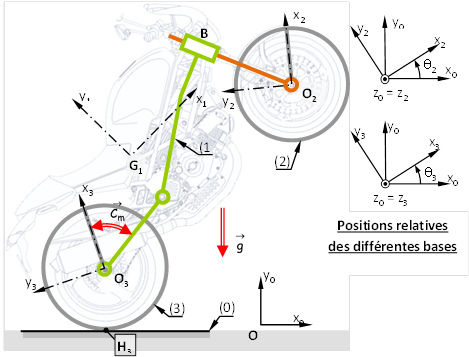
\includegraphics[width=\linewidth]{fig_01}
\end{marginfigure}
\begin{marginfigure}
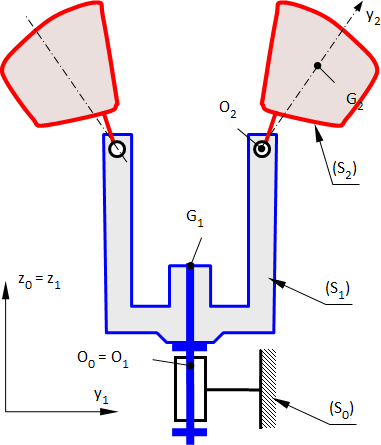
\includegraphics[width=\linewidth]{fig_02}
\end{marginfigure}
\else

\begin{figure*}[!h]
\centering
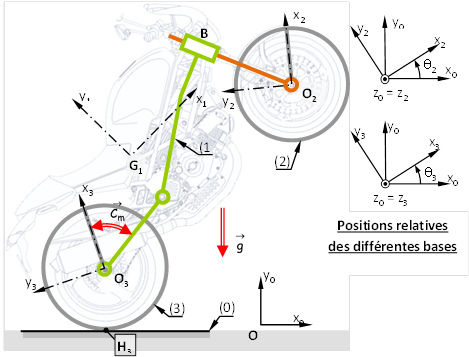
\includegraphics[width=.6\linewidth]{fig_01}
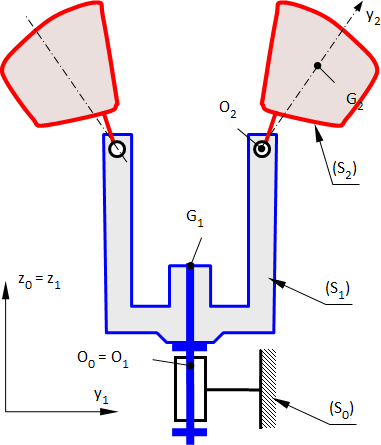
\includegraphics[width=.35\linewidth]{fig_02}
\end{figure*}
\fi

\ifprof
\else
\begin{marginfigure}
\centering

\includegraphics[width=3cm]{Cy_04_02_Colle_02_Disque_qr}
\end{marginfigure}
\fi


\question{Déterminer la forme de la matrice d'inertie du cylindre en C dans la base $\mathcal{B}_1'$.}

\question{Déterminer les éléments de réduction en $A$ du torseur dynamique de \textbf{(1)} dans son mouvement par rapport à $\mathcal{R}_0$.}

\question{Appliquer le PFD pour déterminer les inconnues de liaison.}




\ifprof
\begin{center}
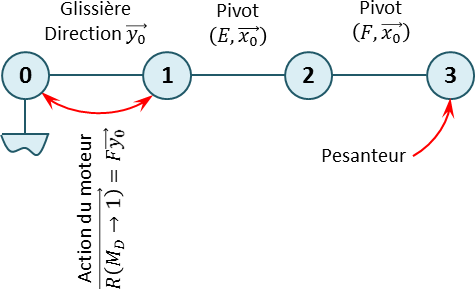
\includegraphics[width=\linewidth]{cor_01}
\end{center}
\begin{center}
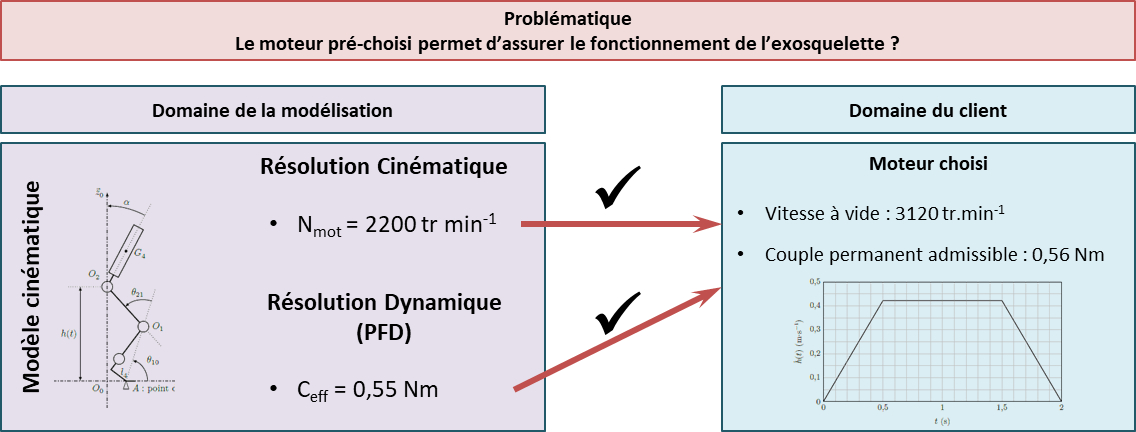
\includegraphics[width=\linewidth]{cor_02}
\end{center}
\begin{center}
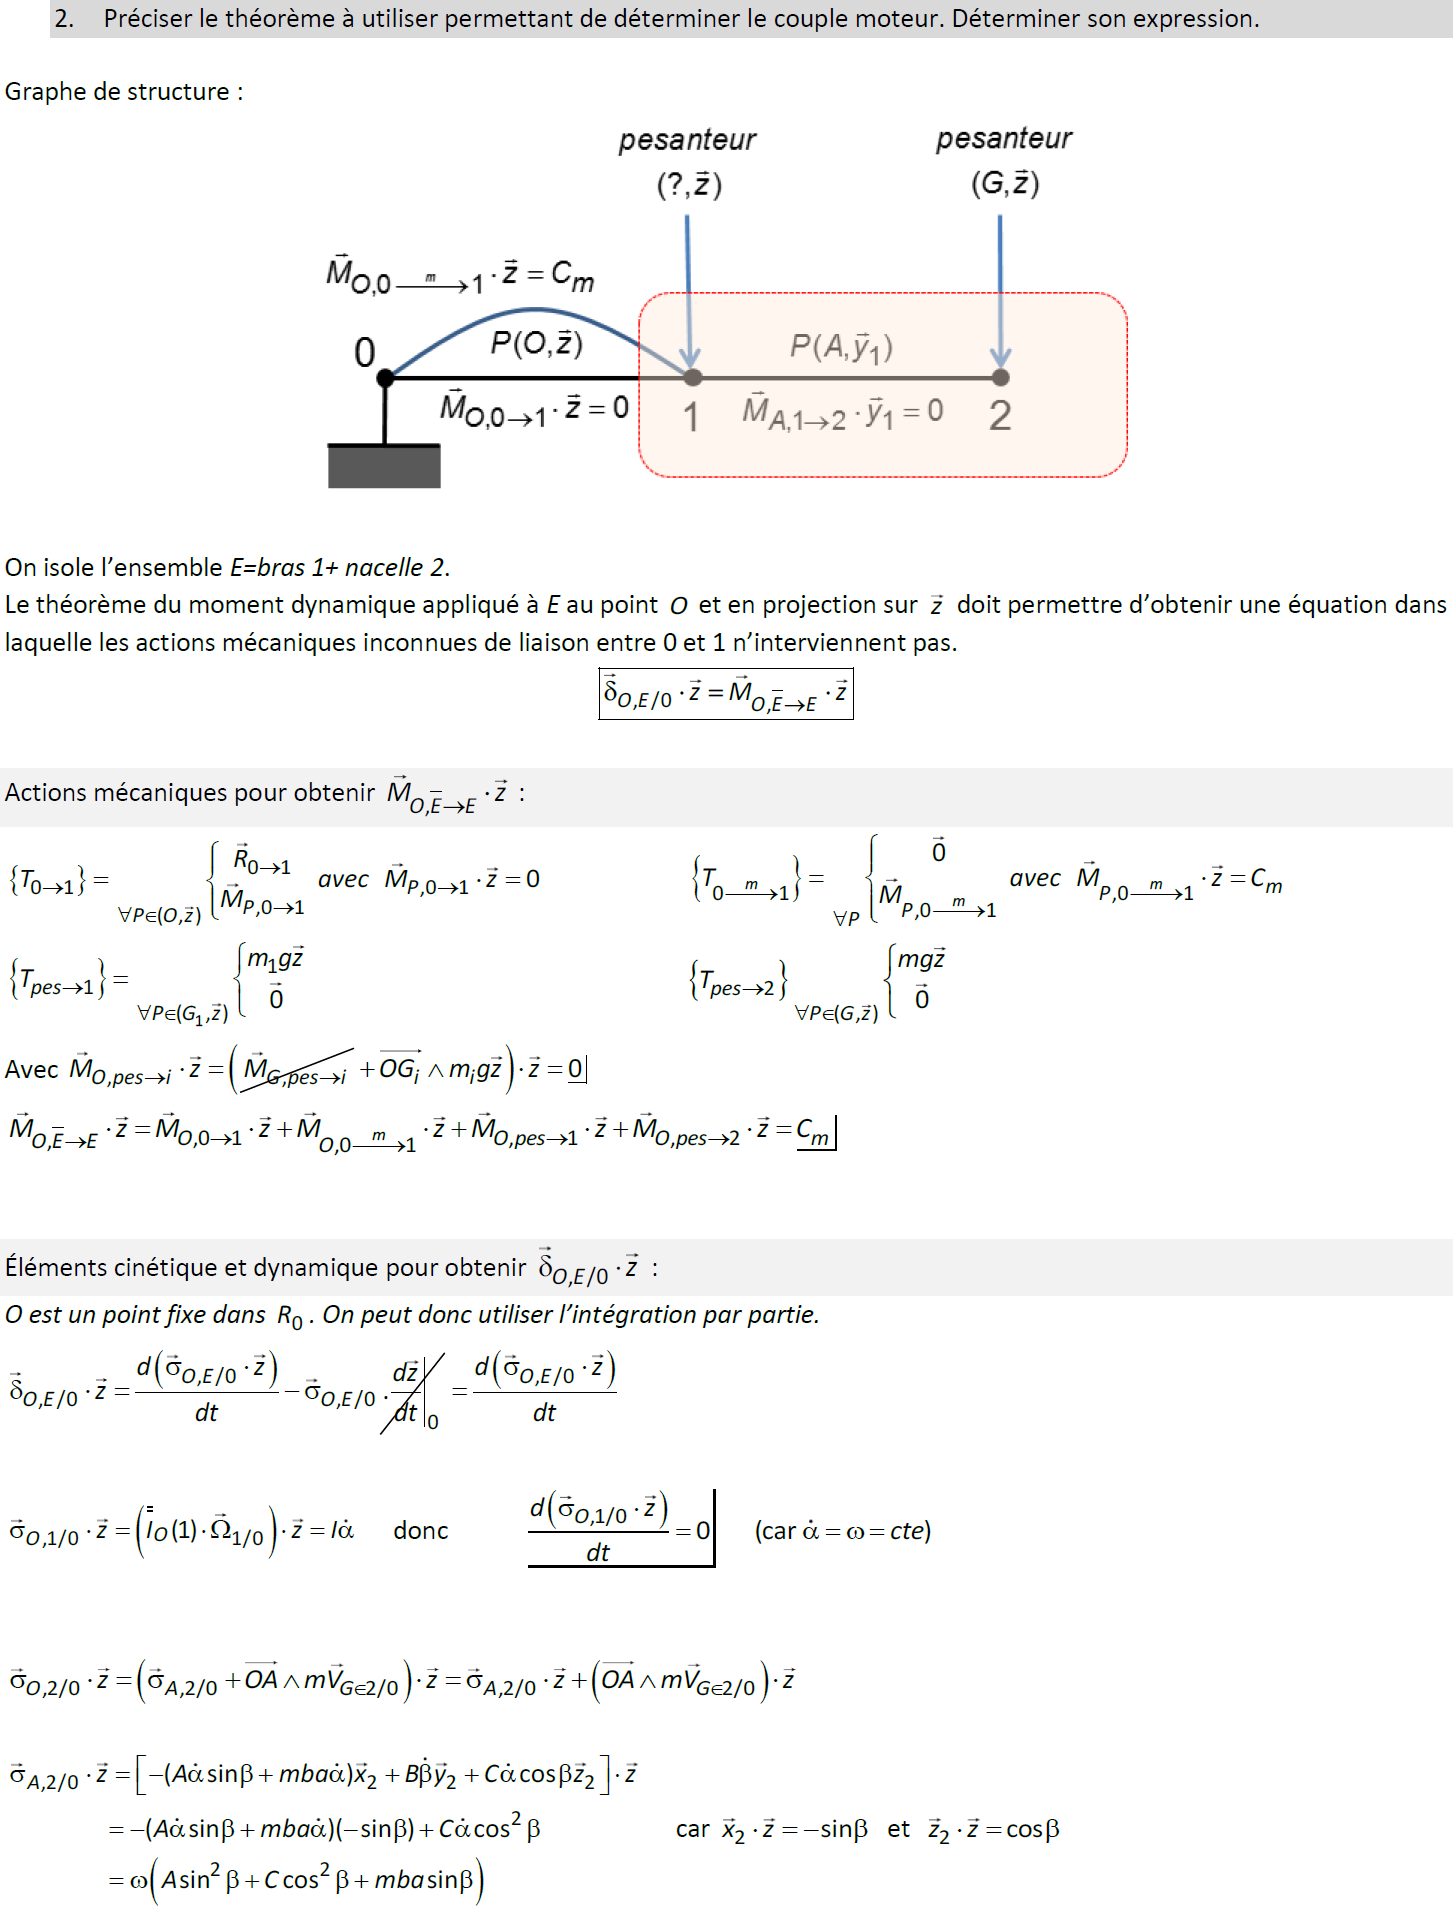
\includegraphics[width=\linewidth]{cor_03}
\end{center}
\begin{center}
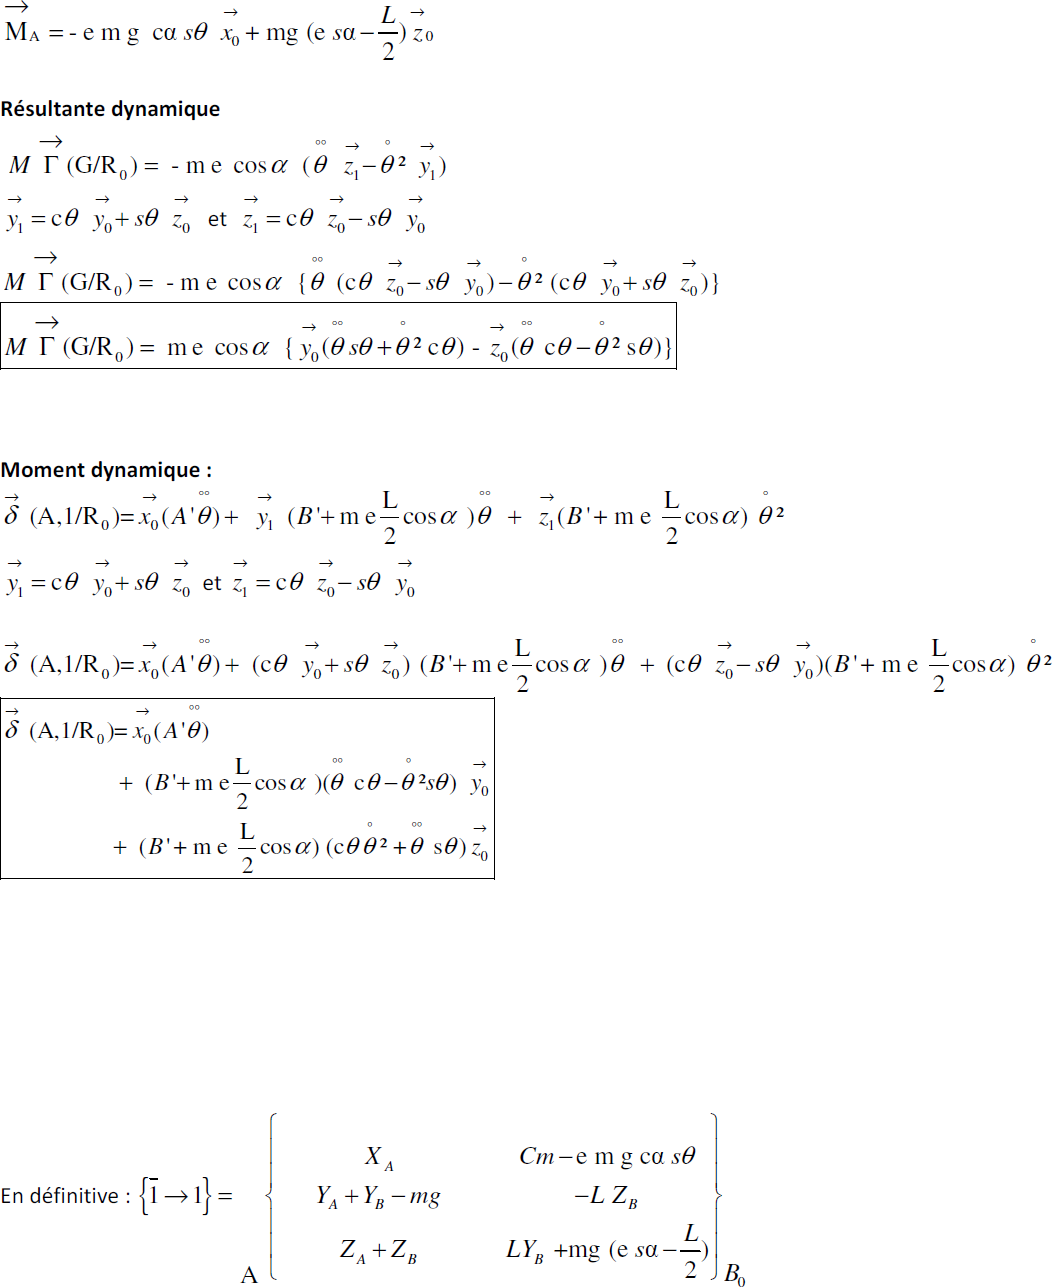
\includegraphics[width=\linewidth]{cor_04}
\end{center}
\begin{center}
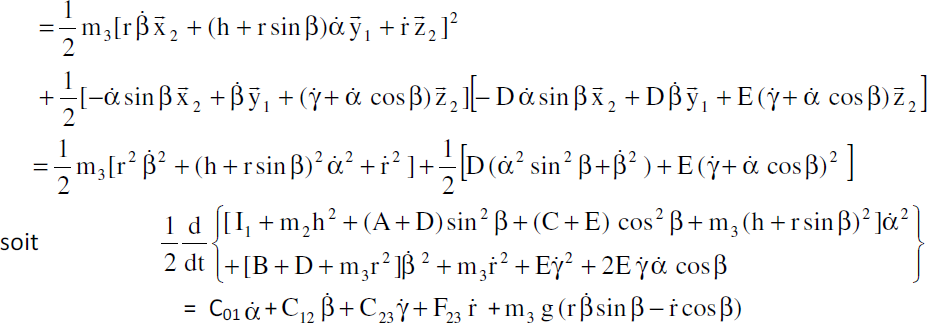
\includegraphics[width=\linewidth]{cor_05}
\end{center}

\else
\fi

